\subsection{单循环链表}

\begin{frame}\ft{\secname}
\begin{dingyi}[单循环链表]
单循环链表是一种头尾相连的链表。
\end{dingyi}
%%%%%%%%%%%
\vspace{0.1in}\pause 

\textcolor{acolor5}{特点:}
尾结点的指针域指向头结点,整个链表的指针域链接成一个环。
%%%%%%%%%%%
\vspace{0.1in}\pause 
 
\textcolor{acolor5}{优点:}
从单循环链表的任意一个结点出发都可以找到其它结点,使得表的处理更加方便灵活。
\end{frame}

\begin{frame}\ft{\secname}
\begin{figure}
\centering
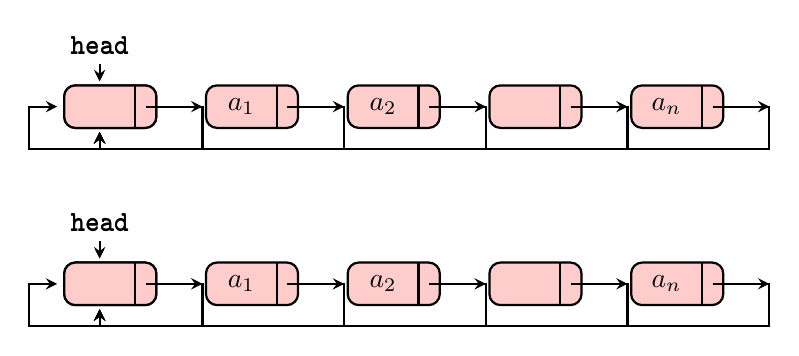
\begin{tikzpicture}[scale=0.9]
\def \x{1}
\def \y{0.6}

\foreach \c in {0,2.5}{
\ifthenelse{ 0 = \c}{
\foreach \r in {0,2,4,6,8}{
\ifthenelse{  6 = \r }{
\node[left] at (\r+\x,\c+0.5*\y) {$\cd$};
}{
\draw[thick,fill=red!20,rounded corners](\r+0,\c+0)rectangle(\r+1.3*\x,\c+\y);  
\draw[thick](\r+\x,\c+0)--(\r+\x,\c+\y); 
}
\ifthenelse{ 8 = \r}{
\draw[thick,->,>=stealth] (\r+1.15*\x,\c+0.5*\y)
--(\r+1.95*\x,\c+0.5*\y)
--(\r+1.95*\x,\c-0.5*\y)
--( 0+0.5*\x,\c-0.5*\y)
--( 0+0.5*\x,\c-0.1*\y);
}{
\draw[thick,->,>=stealth] (\r+1.15*\x,\c+0.5*\y)
--(\r+1.95*\x,\c+0.5*\y);}
}

\node[]at(2.5,\c+0.5*\y){$a_1$};
\node[]at(4.5,\c+0.5*\y){$a_2$}; 
\node[]at(8.5,\c+0.5*\y){$a_n$};
\draw[->,>=stealth] (0.5,\c+1.5*\y)node[above] {\tt head} --(0.5,\c+1.1*\y);
%\node[left=0.5]at( 0-0.5*\x,\c+0.5*\y){空表};
}{
\foreach \r in {0}{
\draw[thick,fill=red!20,rounded corners](\r+0,\c+0)rectangle(\r+1.3*\x,\c+\y);  
\draw[thick](\r+\x,\c+0)--(\r+\x,\c+\y);
\draw[thick,->,>=stealth] (0.5,\c+1.5*\y)node[above] {\tt head} --(0.5,\c+1.1*\y);

\draw[thick,->,>=stealth] (\r+1.15*\x,\c+0.5*\y)
--(\r+1.95*\x,\c+0.5*\y)
--(\r+1.95*\x,\c-0.5*\y)
--( 0-0.5*\x,\c-0.5*\y)
--( 0-0.5*\x,\c+0.5*\y)
--( 0-0.1*\x,\c+0.5*\y);
}
%\node[left=0.5]at( 0-0.5*\x,\c+0.5*\y){非空表};
}
}

\end{tikzpicture}
\caption{单循环链表示意图}
\end{figure}

\end{frame}
%
%
%
\begin{frame}[fragile]\ft{单循环链表的操作}
对单循环链表,除链表的合并外,其它操作和单链表基本一致,仅需在单链表的算法基础上作以下简单修改:
\begin{itemize}
\item[(1)]
判断是否为空链表:
\begin{lstlisting} 
head->next == head;
\end{lstlisting}
\item[(1)]
判断是否为表尾结点:
\begin{lstlisting} 
p->next == head;
\end{lstlisting}
\end{itemize}•
\end{frame}